%----------------------------------------------------------------
%
%  File    :  chapter3.tex
%
%  Authors :  Michael Fuska, FH Campus Wien, Austria
% 
%  Created :  08 Feb 2016
% 
%  Changed :  
% 
%----------------------------------------------------------------
\chapter{Mobiles Betriebssystem von Apple: iOS}
\label{ch:iOS}
%------------------------------------------------------------------------------
%---------------------------------- iOS Grundlagen
\section{iOS Grundlagen}
\label{sec:iOSGrundlage}

Das mobile Apple Betriebsystem iOS basiert auf dem Desktop Betriebssystem des
Mac OS X. Darwin ist ein frei erhältliches Linux basiertes Betriebssystem.
Dieses Betriebssystem stellt die Grundlage für das Mac OS X dar. 
Der Kernel des Mac OS X ist der XNU-Kernel mit entsprechenden Adaptionen für
das Mac OS X und dem mobilen Betriebssystem iOS.
\begin{figure}[htbp]
        \centering
                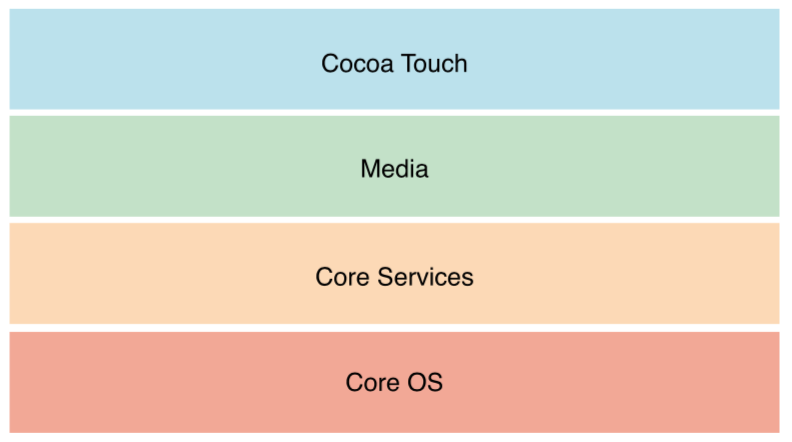
\includegraphics[height=5cm]{Bilder/Chapter3_SystemArchitektur}
        \caption{iOS Software Layer\cite{Apple[6]}}
        	\label{fig:iOS Software Layer}
\end{figure}
Die abgebildeten Schichten zeigen das abstrahiert iOS Betriebssystem. Der
grösste Unterschied zwischen Mac OS X und iOS liegt im Cocoa Touch Layer.
  
\begin{description}
\item[Folgende \glqq Anforderungen\grqq{} werden an das iOS Software Layer
Modell gestellt]~\par
	\begin{itemize}
		\item Sicherstellungen der \textbf{Datenintegrität}
		\item Gewährleistung der \textbf{Informationsvertraulichkeit}
		\item Sicherstellung der \textbf{User- und/oder Applikation Authentizität}
		\item Gewährleistung der \textbf{Daten/Informationsverbindlichkeit}
	\end{itemize}
\end{description}

%------------------------------------------------------------------------------
%---------------------------------- iOS Software Layer

\section{iOS Software Layer}
\label{sec:iOSSWLayer}

%---------------------------------- Core OS ------------------------------------
\subsection{Core OS Layer}
\label{sec:CoreLayer}

Der Core OS Layer beinhaltet alle \glqq low-level\grqq{} Features und auf
diesen bauen alle anderen Frameworks auf. iOS Applikationsentwickler kommen mit
diesem Layer nur dann in Berührung, wenn sie sich mit der Sicherheit und mit
Hardware-Kommunikation beschäftigen. Dieser Layer stellt folgende
\begin{description}
	\item[\glqq Frameworks\grqq{}]zu Verfügung~\par
	\begin{itemize}
		\item Accelerate Framework
		\item Core Bluetooth Framework
		\item External Accessory Framework
		\item Generic Security Service Framework
		\item Lost Authentication Framework
		\item Network Extension Framework
		\item Security Framework
		\item System
		\item 64-Bit Support
	\end{itemize}
\end{description}
 (vgl. \cite{Apple[6]}, S.49-52)
%---------------------------------- Core Service
\subsection{Core Service Layer}
\label{sec:CoreServiceLayer}		
Der \glqq Core Service Layer\grqq{} beinhaltet die fundamentalen System
Service. Dieser Layer wird unterteilt in \glqq high-level\grqq{} Feature und
Core Services Frameworks.
\begin{description}
	\item[\glqq high-level\grqq{} Feature]~\par
	\begin{itemize}
		\item Peer-to-Peer Services
		\item iCloud Storage
		\item Block Objects
		\item Data Protection
		\item File-Sharing Support
		\item Grand Central Dispatch
		\item In-App Purchase
		\item SQLite
		\item XML Support 
	\end{itemize}
	\item[\glqq Core Services Framework\grqq{}]~\par
	\begin{multicols}{2}
	\begin{itemize}
		\item Accounts Frameworks
		\item Address Book Framework
		\item Ad Support Framework
		\item CFNetwork Framework
		\item CloudKit Framework
		\item Core Data Framework
		\item Core Foundation Framework
		\item Core Location Framework
		\item Core Media Framework
		\item Core Motion Framework
		\item Core Telephony Framework
		\item EvenKit Framework
		\item Foundation Framework
		\item HealthKit Framework
		\item HomeKit Framework
		\item JavaScript Framework
		\item Mobile Core Services Framework
		\item Multipeer Connectivity Framework
		\item NewStandKit Framework
		\item PassKit Framework
		\item Quick Look Framework
		\item Safari Services Framework
		\item Social Framework
		\item StoreKit Framework
		\item System Configuration Framework
		\item WebKit Framework
	\end{itemize}
	\end{multicols}
\end{description}
(vgl. \cite{Apple[6]}, S.36-48)
%---------------------------------- Media Layer
\subsection{Media Layer}
\label{sec:MediaLayer}		
In diesem Layer sind alle Technologien zur Darstellung von Grafik, Video und
Sound enthalten. Dieser Layer ist verantwortlich für das Design und den Sound
der iOS Applikationen.
Dieser Layer stellt folgende
\begin{description}
	\item[\glqq Technologien\grqq{}]zur Verfügung~\par
	\begin{itemize}
		\item Graphics Technologies
		\item Audio Technologies
		\item Video Technologies
		\item AirPlay
	\end{itemize}
\end{description}

\begin{description}
	\item[Folgende Frameworks beinhaltet dieser Layer]~\par
	\begin{multicols}{2}
	\begin{itemize}
		\item Assets Library Framework
		\item AV Foundation Framework
		\item AVKit Framework
		\item CoreAudioKit Framework
		\item Core Graphics Framework
		\item Core Image Framework
		\item Core Text Framework
		\item Core Video Framework
		\item Game Controller Framework
		\item GLKit Framework
		\item Image I/O Framework
		\item Media Accessibility Framework
		\item Media Player Framework
		\item Metal Framework
		\item OpenGL ES Framework
		\item Photos Framework
		\item Photos UI Framework
		\item Quartz Core Framework
		\item SceneKit Framework
		\item SpriteKit Framework
         \end{itemize}
	\end{multicols}
\end{description}
(vgl. \cite{Apple[6]}, S.23-35)
%---------------------------------- Cocoa Touch Layer
\subsection{Cocoa Touch Layer}
\label{sec:CocoaTouchLayer}
Enthält die wichtigsten Frameworks um iOS Applikationen zu entwickeln. Dieser
Layer stellt die Basis Applikation Infrastruktur und folgende
\begin{description}
\item[\glqq Key Technologien\grqq{}]zu Verfügung ~\par  
	\begin{itemize}
		\item Multitasking
		\item touch-based input
		\item push notification
		\item \glqq high-level\grqq{} System Service
	\end{itemize}
\end{description}

\begin{description}
\item[Folgende Features sind in diesem Layer enthalten]~\par
	\begin{multicols}{2}
	\begin{itemize}
		\item App Extentision
		\item Handoff
		\item Document Picker
		\item AirDrop
		\item TextKit
		\item UIKit Dynamics
		\item Multitasking
		\item Auto Layout
		\item Storyboards
		\item UI State Preservation
		\item Apple Push Notification Service
		\item Local Notifications
		\item Gesture Recognizers
		\item Standard System View Controllers
         \end{itemize}
	\end{multicols}
\end{description}

\begin{description}
	\item[Folgende Frameworks beinhaltet dieser Layer]~\par
	\begin{multicols}{2}
	\begin{itemize}
		\item Address Book UI Framework
		\item EventKit UI Framework
		\item GameKit Framework
		\item iAd Framework
		\item MapKit Framework
		\item Message UI Framework
		\item Notification Center Framework
		\item PushKit Framework
		\item Twitter Framework
		\item UIKit Framework
         \end{itemize}
	\end{multicols}
\end{description}
(vgl. \cite{Apple[6]}, S.12-22)

%---------------------------------- iOS Device Security Architektur
\pagebreak
\section{iOS Device Security Architektur}
\label{sec:iOSSecArchitektur}

Der Sicherheitsmechanismus der iOS Device unterteilt sich in zwei Ebenen. 
\begin{figure}[htb]
  \begin{minipage}{0.6\textwidth} 
  		\begin{description}
   			\item[ iOS Sicherheitsebenen]~\par
         		\begin{enumerate}	
				\item  \textbf{iOS Software}
					\begin{enumerate}
       						\item File System
         					\item OS Partition
						\item User Partition (verschlüsselt)
						\item App Sandbox
						\item Data Protection Class
      					\end{enumerate}
      				\item  \textbf{iOS Hardware und Firmware}~\par
					\begin{enumerate}
       						\item Kernel
						\begin{enumerate}
						\item Secure Enclave
						\item Secure Element
         					\end{enumerate}	
						\item Crypto Engine
						\item Device Key
						\item Group Key
						\item Apple Root Certificate
      					\end{enumerate}
			\end{enumerate}
   		\end{description}
Die iOS Sicherheit passiert auf der Kombination von Software, Hardware und
Services um ein maximum an Sicherheit zu erreichen. (vgl. \cite{Apple[4]}, S.4)
	\end{minipage}
	\hfil
	\begin{minipage}{0.4\textwidth}
		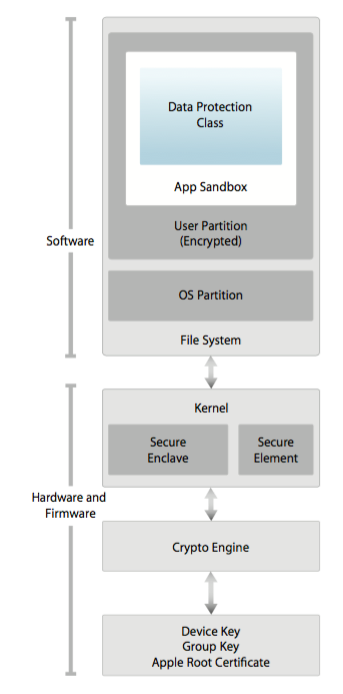
\includegraphics[width=\textwidth]{Bilder/Chapter3_SecArchitektur}
		\caption {iOS Security Architektur \cite{Apple[4]}}
        \label{fig:iOS Security Architektur}
	\end{minipage}
\end{figure}
		    	
%---------------------------- System Security
\subsection{System Security}
\label{sec:SystemSec}
Apple hat die System Security so entwickelt, dass Software und Hardware für
jedes iOS Device sicher sind, über alle Kernkomponenten des iOS Devices.
Dies beinhaltet den sicheren Boot Prozess (inklusive Boot Chain), die Software
Updates und die \glqq Secure Enclave\grqq. Alle die Maßnahmen dienen dazu, um
zu gewährleisten, dass nur \glqq vertrauenswürdige Applikation \grqq{} auf dem
iOS Device ausgeführt werden können.\\
Die enge Verbindung zwischen Hardware und Software der iOS Geräte
gewährleistet, dass alle Komponenten des Systems \glqq vertrauenswürdig\grqq{}
sind, sowohl die Software als auch die Hardware.
 (vgl. \cite{Apple[4]}, S.5)
\begin{description}
\item[Apple führt unter dem Kapitel \glqq System Security\grqq{}  folgende
Features an:]~\par
	%\begin{multicols}{2}
	\begin{itemize}
		\item Secure Boot Chain (siehe Kapitel:\ref{sec:SecBootChain})
 		\item System Software Authorization
 		\item Secure Enclave
 		\item Touch ID
        \end{itemize}
	%\end{multicols}
\end{description}
(vgl. \cite{Apple[4]}, S.5-9)

%--------------------------- Encryption und Daten Sicherheit
\subsection{Encryption und Daten Sicherheit}
Das iOS unterstützt standardmäßig eine Verschlüsselung und
Datenschutzfunktionen für persönliche- und Unternehmensdaten.
Die Sicherheitsinfrastruktur des iOS Devices ist so aufgebaut, dass selbst wenn
ein Teil des Betriebsystem kompromittiert ist, die anderen Bereiche des
Devices, weiterhin sicher vor unerlaubten Zugriff sind. \\
Dies ist besonders für Unternehmen wichtig, da dadurch gewährleistet ist, dass
vertrauliche Unternehmensdaten nicht gelesen werden können. Weitere iOS
Features stellen sicher, dass selbst bei Diebstahl oder Verlust des iOS Devices
die Daten sicher sind.
Alle diese Features sind in der Standardkonfiguration eingeschalten.

\label{sec:DataEnc}
\begin{description}
\item[\parbox{\textwidth} {Apple führt unter dem Kapitel \glqq Encryption und
Daten Sicherheit\grqq{} folgende Features an:}]~\par
	\begin{multicols}{2}
	\begin{itemize}
		\item Hardware Security Features
 		\item File Data Protection
 		\item Passcodes
 		\item Data Protection Classes
		\item Keychain Data Protection
		\item Access to Safari saved Password
		\item Keybags
		\item Security Certification and programs
        \end{itemize}
	\end{multicols}
\end{description}
(vgl. \cite{Apple[4]}, S.10-17)

%------------------------------ Applikation Security
\subsection{Applikation Security}
\label{sec:AppSec}
Applikationen sind das größte Sicherheitsrisiko für ein Betriebssystem. Das
Verhalten des Betriebssystems kann durch Applikationen negativ beeinflusst
werden.
Es kann die Sicherheit und die Verfügbarkeit des iOS Devices beeinträchtigen. 
Des weiter kann die Integrität des Benutzerdaten durch unsicher Applikationen
gefährdet werden.
\begin{description}
\item[\parbox{\textwidth} {Apple führt unter dem Kapitel \glqq Applikation
Security\grqq{} folgende Features an:}]~\par
	\begin{multicols}{2}
	\begin{itemize}
		\item App Code signing
		\item Runtime process security
		\item Extensions
		\item App Groups
		\item Data Protection in apps
		\item Accessories
		\item HomeKit
		\item HealthKit
		\item Apple Watch
        \end{itemize}
	\end{multicols}
\end{description}
(vgl. \cite{Apple[4]}, S.18-26)

%------------------------------ Network Security
\subsection{Network Security}
\label{sec:NetworkSec}
Die Netzwerk Sicherheit ist ein wichtiger Bestandteil des Sicherheitskonzept
von Apple und ergänzt die integrierten iOS Sicherheitsmechanismen.
Die integrierten Sicherheitsmechanismen die iOS Devices dienen dazu um die
Daten auf dem Device zu schützen.
Das iOS Device muss in der Lage sein, Weltweit auf die Daten zugreifen zu
können. Dieser Zugriff muss so abgesichert sein, dass die Übertragung der Daten
sicher ist.
Es werden vom iOS Standard Netzwerkprotokolle für eine authentifizierte,
autorisierte und verschlüsselte Kommunikation verwendet.
\begin{description}
\item[\parbox{\textwidth} {Apple führt unter dem Kapitel \glqq Network
Security\grqq{} folgende Netzwerksicherheit Protokolle und Architekturen
an:}]~\par
	\begin{itemize}
		\item Virtual Private Network (VPN)
 		\item Transport Layer Security (TLS) (siehe Kapitel:\ref{sec:TLS})
		\item Single Sign-on
        \end{itemize}
\end{description}
Des weiter werden die neuersten Standards für WLAN, Bluetooth und
Mobilfunkverbindungen verwendet. (vgl. \cite{Apple[4]}, S.27-30)

%------------------------------ Apple Pay ----------------------------------
\subsection{Apple Pay}
\label{sec:ApplePay}

\begin{description}
\item[\parbox{\textwidth} {Folgende Komponenten gehören zum \glqq Apple
Pay\grqq{} Produkt}]~\par
	\begin{itemize}
		\item Secure Element \\
Die Secure Element erfüllen den Industriestandard . Der zertifizierte Chips
werden ein einer Java Card Plattform ausgeführt.
		Diese Elemente erfüllen Finanzindustrie Standard. 
 		\item Near Field Communication (NFC ) Controller \\
Der NFC Controller und die NFC Kommunikation Protokolle sind für die
Kommunikation zwischen den Anwendungsprozessoren und Secure Elementen zuständig.
 		\item Wallet \\
Wallet ist Apples Applikation,  welche für die Verwaltung der Kreditkarten und
Debitkarten verantwortlich ist. Diese Applikation ist für die Ausführung der
Finanztransaktionen verwantwortlich.
 		\item Secure Enclave \\
Die \glqq Secure Enclave\grqq{} ist für den Authentifizierungsprozess einer
Finanztransaktion zuständig. Des weiter werden in der  \glqq Secure
Enclave\grqq{}  die Fingerabdrücke für die Touch-ID gespeichert.
 		% \item Apple Pay Servers \\		
        \end{itemize}
\end{description}
(vgl. \cite{Apple[4]}, S.31-37)
%------------------------------ Internet services
\subsection{Internet Services}
\label{sec:InternetServices}

Apple hat sehr stabile Applikationen für den Benutzer von iOS Geräten
entwickelt wie zum Beispiel: iMessage, Facetime, iCloud und iCloud Keychain. 

Für die Internet Dienste stehen den Entwicklern die selben
Sicherheitsmechanismen zur Verfügung. Natürlich gelten für Internet Dienste die
selben Sicherheitsziele, wie für die Apple internen Produkte. 
Diese Ziele beinhalten den sicheren Umgang mit den persönlichen Daten der
Benutzer, sowie den Schutz vor nicht autorisierten Zugriff auf die persönlichen
Daten des Benutzers und anderer Dienstleistungen.
Jeder Dienst verwendet eine eigene leistungsstarke Sicherheitsarchitektur ohne
die Benutzerfreundlichkeit des gesamten iOS Devices zu beeinträchtigen. (vgl.
\cite{Apple[4]}, S.38-49)

\begin{description}
    \item[\parbox{\textwidth} {Dies sind die Mainfeatures des Apple \glqq
        Internet Service \grqq{}}]~\par
    \begin{itemize}
        \item Apple ID
        \item iCloud
        \item iCloud Keychain
        \item Continuity \\
        Darunter versteht Apple, dass Verteilen von verschieden Informationen
über mehrere iOS Devices.
    \end{itemize}

\end{description}

%------------------------------ Device Controls

\subsection{Device Controls}
\label{sec:DeviceControl}
(vgl. \cite{Apple[4]}, S.50-55)
%----------------------------- Privacy Controls

\subsection{Privacy Controls}
\label{sec:}
(vgl. \cite{Apple[4]}, S.56)